% Technical report of the Python implementation of Stage 1.
% Build from python/stage_1/docs/report/:
%   python charts.py      (figures/*.pdf and tables/*.tex, from ../../benchmarks/results/)
%   python compare.py     (figures/lang_*.pdf and tables/lang_summary.tex, the three languages)
%   pdflatex report.tex && pdflatex report.tex     (twice, for the table of contents)
% A figure or table that does not exist yet shows a red \pending box, so the report always compiles.
\documentclass[11pt,a4paper]{article}

\usepackage[utf8]{inputenc}
\usepackage[T1]{fontenc}
\usepackage{lmodern}
\usepackage{microtype}
\usepackage[margin=2.4cm,headheight=14pt]{geometry}
\usepackage{graphicx}
\usepackage{booktabs}
\usepackage{tabularx}
\usepackage{longtable}
\usepackage{array}
\usepackage{enumitem}
\usepackage{float}
\usepackage{xcolor}
\usepackage{listings}
\usepackage{tikz}
\usetikzlibrary{positioning,arrows.meta,fit,calc}
\usepackage{fancyhdr}
\usepackage{titlesec}
\usepackage[hidelinks]{hyperref}

\definecolor{accent}{HTML}{2a78d6}
\definecolor{ink}{HTML}{0b0b0b}
\definecolor{muted}{HTML}{52514e}
\definecolor{codebg}{HTML}{f6f6f4}
\definecolor{rule}{HTML}{d8d7d2}
\definecolor{notebg}{HTML}{eef4fc}
\definecolor{pendingred}{HTML}{c62828}

\hypersetup{colorlinks=true,linkcolor=accent,urlcolor=accent,citecolor=accent}

\titleformat{\section}{\Large\bfseries\color{ink}}{\thesection.}{0.6em}{}
\titleformat{\subsection}{\large\bfseries\color{ink}}{\thesubsection}{0.6em}{}
\titleformat{\subsubsection}{\normalsize\bfseries\color{ink}}{\thesubsubsection}{0.6em}{}
\titlespacing*{\section}{0pt}{1.6em}{0.7em}
\titlespacing*{\subsection}{0pt}{1.2em}{0.5em}

\pagestyle{fancy}
\fancyhf{}
\fancyhead[L]{\small\color{muted}Stage 1 $\cdot$ Data layer $\cdot$ Python implementation}
\fancyhead[R]{\small\color{muted}Big Data $\cdot$ ULPGC}
\fancyfoot[C]{\small\thepage}
\renewcommand{\headrulewidth}{0.4pt}

\setlist{itemsep=2pt,topsep=4pt}
\setlength{\parskip}{0.45em}
\setlength{\parindent}{0pt}
\setlength{\emergencystretch}{3em}   % long \texttt names: stretch spaces rather than overflow
\renewcommand{\arraystretch}{1.25}

\lstdefinestyle{python}{
  language=Python, basicstyle=\ttfamily\footnotesize, backgroundcolor=\color{codebg},
  keywordstyle=\color{accent}\bfseries, commentstyle=\color{muted}\itshape,
  stringstyle=\color{ink}, frame=single, rulecolor=\color{rule}, framesep=4pt,
  xleftmargin=6pt, xrightmargin=6pt, breaklines=true, columns=fullflexible,
  keepspaces=true, showstringspaces=false, aboveskip=8pt, belowskip=8pt}
\lstdefinestyle{shell}{
  language={}, basicstyle=\ttfamily\footnotesize, backgroundcolor=\color{codebg}, frame=single,
  rulecolor=\color{rule}, framesep=4pt, xleftmargin=6pt, xrightmargin=6pt,
  breaklines=true, columns=fullflexible, keepspaces=true, showstringspaces=false,
  aboveskip=8pt, belowskip=8pt, literate={í}{{\'i}}1 {ó}{{\'o}}1 {á}{{\'a}}1}
\lstset{style=python}

\newcolumntype{Y}{>{\raggedright\arraybackslash}X}
\newcommand{\code}[1]{\texttt{#1}}
\newcommand{\us}{\,$\mu$s}
\newenvironment{note}{\par\smallskip\noindent
\begin{tikzpicture}\node[fill=notebg,draw=accent!40,rounded corners=2pt,inner sep=7pt,text width=\dimexpr\linewidth-14pt\relax]\bgroup\small}{\egroup;\end{tikzpicture}\par\smallskip}

% One module card in the code walkthrough: \cls{name}{kind}
\newcommand{\cls}[2]{\par\medskip\noindent{\large\bfseries\code{#1}}\hspace{0.6em}{\small\color{muted}#2}\par\nopagebreak\smallskip}
\newcommand{\why}[1]{\par\noindent\textit{Design rationale.} #1\par}

% Text that can only be written once the benchmark results are committed.
\newcommand{\pending}[1]{{\color{pendingred}\bfseries[Pending: #1]}}
% \detokenize: the file names contain underscores, which would break the \pending text.
\newcommand{\pythonfigure}[2]{\IfFileExists{figures/#1.pdf}{\includegraphics[width=#2]{figures/#1.pdf}}{\pending{figure \detokenize{#1}}}}
\newcommand{\pythontable}[1]{\IfFileExists{tables/#1.tex}{\input{tables/#1}}{\pending{table \detokenize{#1}}}}

\begin{document}

% ---------------------------------------------------------------- title page
\begin{titlepage}
\thispagestyle{empty}
\vspace*{2.5cm}
{\color{accent}\rule{\linewidth}{1.2pt}}\\[0.8cm]
{\Huge\bfseries Search Engine Project\par}
\vspace{0.4cm}
{\LARGE Stage 1: Building the Data Layer\par}
\vspace{0.6cm}
{\Large\color{muted} Python implementation --- technical report\par}
\vspace{0.6cm}
{\color{accent}\rule{\linewidth}{1.2pt}}
\vspace{2cm}

\begin{tabular}{@{}>{\bfseries}p{3.4cm}p{10.5cm}@{}}
Course & Big Data $\cdot$ Grado en Ciencia e Ingeniería de Datos $\cdot$ Universidad de Las Palmas de Gran Canaria \\
Academic year & 2026/2027 \\
Group name & BigData-Ulpgc \\
Members & Daniel Perdomo Medina --- Python implementation, author of this report \\
 & Daniel Rodríguez Alonso --- Java implementation \\
 & Carlos Falcón Brito --- C++ implementation \\
Repository & \url{https://github.com/BigData-Ulpgc/stage_1}, branch \code{main}, folder \code{python/stage\_1/} \\
Status & Complete pipeline writing the three datalakes and the three indexes, offline mode with the sample dataset, 12 benchmark experiments, 39 tests passing \\
Date & 4 October 2026 \\
\end{tabular}

\vfill
\begin{note}
\textbf{Quick check for instructors.} From \code{python/stage\_1/}, with Python~3.10+ and no network:
\code{pip install -r ../requirements.txt pytest}, \code{pytest src/test}, then
\code{python -m src.main.bigdata.main pipeline 15 -{}-offline-source ../../sample\_dataset/raw} and
\code{python -m src.main.bigdata.main search whale island}, which finds books 76, 84 and 2701.
Section~\ref{sec:quick} gives the details.
\end{note}
\end{titlepage}

% ---------------------------------------------------------------- abstract + toc
\section*{Abstract}
This report describes the Python implementation of Stage~1 of the group's search engine over
Project Gutenberg books. Stage~1 builds the \emph{data layer}: a pipeline that downloads books,
splits each one into header and body, stores them in a datalake, extracts their metadata into a
SQLite datamart and builds an inverted index that answers Boolean AND queries. A control layer
records the progress, so an interrupted run resumes without losing or repeating books.

The Python pipeline writes every book to the three datalake layouts (\code{book}, \code{range},
\code{time}) and to the three persistent inverted indexes (\code{monolithic} JSON,
\code{hierarchical} folders, \code{mongo}) in the same run. It follows the group's common contract
(\code{shared/SPEC.md}): with the 200 books of the dataset its indexes are byte-for-byte identical
to Java's, and its random sequences reproduce Java's exactly. A 15-book sample dataset lets the
whole pipeline run offline. The 12 benchmark experiments were run on the 200 real books, on the
same Linux machine as the Java ones. \pending{one or two sentences with the main results, once the
CSVs are committed.}

\tableofcontents
\newpage

% ================================================================ 1
\section{Introduction and objectives}

\subsection{Goal of Stage 1}
The course project builds, stage by stage, a search engine over the books of Project Gutenberg.
Stage~1 leaves ranking and user interfaces for later and concentrates on the data underneath it.
The books have to be downloaded and kept, their metadata extracted, and their words indexed. This
has to be done \emph{correctly}, it has to \emph{survive interruptions} without losing or repeating
work, and it has to be \emph{measured}, so that different ways of storing the same data can be
compared with numbers.

\begin{table}[H]
\centering\small
\begin{tabularx}{\linewidth}{@{}l Y l@{}}
\toprule
Layer & What it does & Python package \\
\midrule
Ingestion & Fetches the raw text (Gutenberg or a local folder) and splits it at the START/END markers into header and body; the licence footer is dropped. & \code{crawler} \\
Datalake & Keeps header and body as text files, in three layouts at once: \code{book}, \code{range} and \code{time}. & \code{datalake} \\
Datamarts & Data ready to query: the metadata in SQLite, and the inverted index (term $\rightarrow$ books) in three variants. & \code{datamart.*} \\
Query & AND search: the books that contain every term of the query. & \code{query} \\
Control & Two lists of ids, downloaded and indexed, that let a stopped run continue where it was. & \code{control} \\
Command line & The pipeline loop and the \code{pipeline}, \code{search} and \code{status} commands. & \code{main.py} \\
Benchmarks & The 12 experiments of the SPEC, their checks and the CSV results. & \code{benchmark} \\
\bottomrule
\end{tabularx}
\caption{The layers of the system and where each lives in the Python code.}
\end{table}

\subsection{The group and the common contract}
The same data layer is written three times, in Java, Python (this report) and C++. Results from
three languages can only be compared if the three programs read the same books, process them in
the same way and write the same outputs, so the group wrote a common contract,
\code{shared/SPEC.md}. Everything in it is fixed for the three implementations; everything else is
up to each one.

\begin{table}[H]
\centering\small
\begin{tabularx}{\linewidth}{@{}l Y@{}}
\toprule
SPEC section & What it fixes \\
\midrule
1. Inputs & \code{book\_ids.txt} (the 200 ids, in download order), \code{queries.txt} (the query workload) and \code{stopwords.txt}; blank lines and lines starting with \code{\#} are skipped. \\
2. Split & The START and END markers, with \code{THE} or \code{THIS}; without both, the book is discarded. The header is what comes before START, the body runs from the end of the START line to END, both trimmed, and \code{\textbackslash r\textbackslash n} becomes \code{\textbackslash n}. \\
3. Datalake & The paths of the three layouts: \code{YYYYMMDD/HH/<ID>.body.txt}, \code{<ID>/body.txt} and \code{<START>-<END>/<ID>.body.txt}, with START $= \lfloor ID/1000\rfloor\cdot 1000$ in 5 digits. \\
4. Metadata & Four regexes (title, author, release date, language): first match, first line, trimmed, NULL if absent; the \code{books} table with indexes on \code{author} and \code{title}. \\
5. Tokenizer & Character by character: A--Z is lowered, a--z and 0--9 build tokens, any other character separates; tokens shorter than 2 and stopwords are dropped; a book contributes its \emph{set} of terms. \\
6. Index & \code{inverted\_index.json}, \code{inverted\_index/<LETTER>/<term>.txt} (one id per line) and the Mongo collection \code{inverted\_index}; postings sorted and without duplicates. \\
7. Queries & Same tokenizer; AND = intersection; ids in ascending order. \\
8. Control & \code{downloaded\_books.txt} and \code{indexed\_books.txt}; an id is appended only after its step was written. \\
9--10. Benchmarks & The CSV format, 2 warm-ups + 5 runs, no network inside a measurement, the N books with the lowest ids, the reference term counts, and the generated metadata rows. \\
\bottomrule
\end{tabularx}
\caption{The common contract, \code{shared/SPEC.md}, in short.}
\end{table}

\subsection{Objectives and scope of this report}
The assignment asks for a datalake of raw books, datamarts with the metadata and the inverted
index, a control layer that never loses or duplicates work, and benchmarks of several datalake and
index structures, implemented in at least three languages over the same data.

This report covers the \textbf{Python} implementation. It explains its architecture, the decisions
behind it and each of its modules, how to install, test and run it, and what its benchmarks show,
on their own and next to Java and C++. The other two implementations are described in their own
reports in the repository.

The Python implementation delivers:
\begin{itemize}
  \item The complete pipeline (crawler, datalake, metadata, inverted index, AND search and control
        layer) behind a command line with \code{pipeline}, \code{search} and \code{status}.
  \item The three datalake layouts and the three persistent indexes of the SPEC, all written by the
        same pipeline run, plus an in-memory index used as the reference in the benchmark checks.
  \item An offline source (\code{-{}-offline-source}) that runs the same pipeline on the raw files
        of \code{sample\_dataset/}, without network.
  \item The 12 benchmark experiments of the SPEC in its CSV format, with internal checks that stop a
        run that measures something wrong, and \code{verify\_results}, which checks the CSVs against
        the exact values of SPEC section 10.
  \item 39 \code{pytest} tests.
\end{itemize}

% ================================================================ 2
\section{System architecture}

Figure~\ref{fig:components} follows one book through \code{main.py}. Unlike Java and C++, which
choose one datalake and one index in a configuration file, the Python pipeline writes the book to
every structure in the same pass.

\begin{figure}[H]
\centering
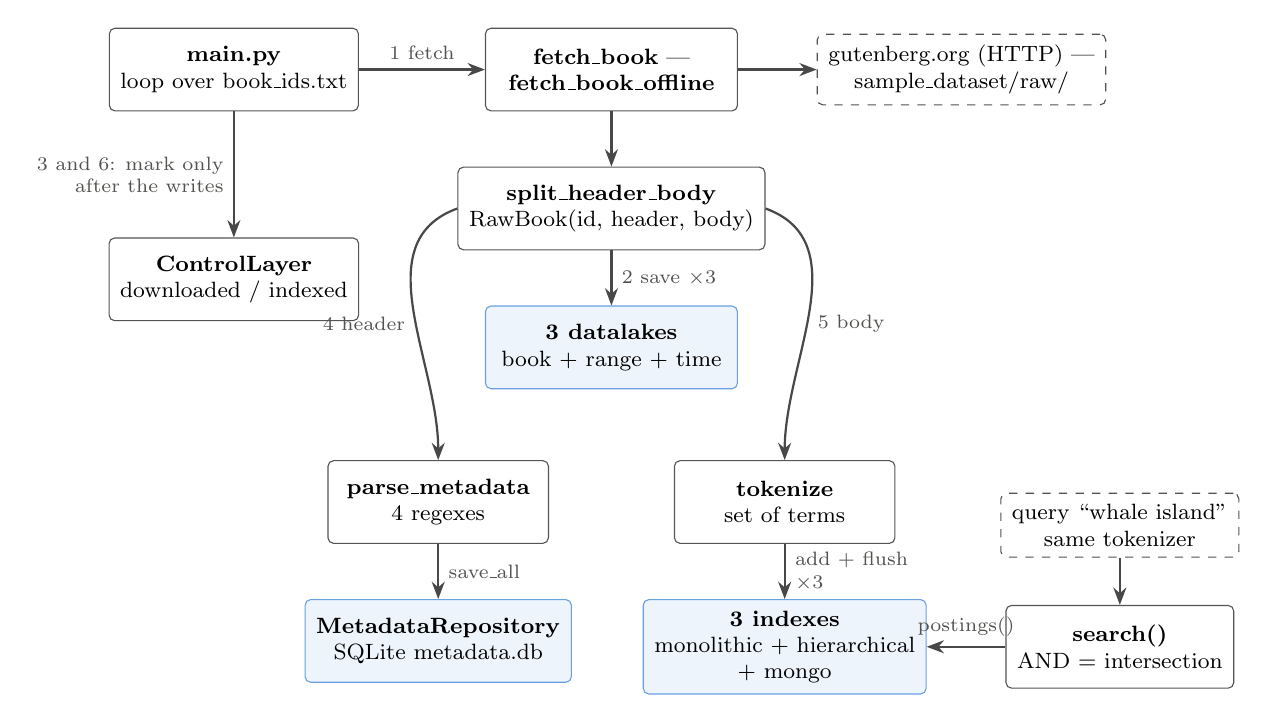
\begin{tikzpicture}[
  font=\footnotesize,
  box/.style={draw=ink!70,rounded corners=2pt,align=center,minimum height=1.05cm,inner sep=4pt,fill=white},
  store/.style={box,fill=notebg,draw=accent!70},
  ext/.style={box,dashed,draw=muted},
  arr/.style={-{Stealth[length=2.2mm]},thick,draw=ink!75},
  lbl/.style={font=\scriptsize,color=muted}]
  \node[box,minimum width=2.8cm] (main) {\textbf{main.py}\\loop over book\_ids.txt};
  \node[box,right=1.6cm of main,minimum width=3.2cm] (fetch) {\textbf{fetch\_book} |\\\textbf{fetch\_book\_offline}};
  \node[ext,right=1.0cm of fetch,minimum width=2.9cm,minimum height=0.8cm] (net) {gutenberg.org (HTTP) |\\sample\_dataset/raw/};
  \node[box,below=0.7cm of fetch,minimum width=3.2cm] (split) {\textbf{split\_header\_body}\\RawBook(id, header, body)};
  \node[store,below=0.7cm of split,minimum width=3.2cm] (lake) {\textbf{3 datalakes}\\book + range + time};
  \node[box,below=1.6cm of main,minimum width=2.8cm] (ctrl) {\textbf{ControlLayer}\\downloaded / indexed};
  \node[box,below=0.9cm of lake,xshift=-2.2cm,minimum width=2.8cm] (parse) {\textbf{parse\_metadata}\\4 regexes};
  \node[box,below=0.9cm of lake,xshift=2.2cm,minimum width=2.8cm] (tok) {\textbf{tokenize}\\set of terms};
  \node[store,below=0.7cm of parse,minimum width=2.8cm] (repo) {\textbf{MetadataRepository}\\SQLite metadata.db};
  \node[store,below=0.7cm of tok,minimum width=3.0cm] (inv) {\textbf{3 indexes}\\monolithic + hierarchical\\+ mongo};
  \node[box,right=1.0cm of inv,minimum width=2.6cm] (ss) {\textbf{search()}\\AND = intersection};
  \node[ext,above=0.6cm of ss,minimum width=2.6cm,minimum height=0.8cm] (q) {query ``whale island''\\same tokenizer};

  \draw[arr] (main) -- node[above,lbl]{1 fetch} (fetch);
  \draw[arr] (fetch) -- (net);
  \draw[arr] (fetch) -- (split);
  \draw[arr] (split) -- node[right,lbl]{2 save $\times$3} (lake);
  \draw[arr] (main) -- node[left,lbl,align=right]{3 and 6: mark only\\after the writes} (ctrl);
  \draw[arr] (split.west) to[out=200,in=90] node[pos=0.55,left,lbl]{4 header} (parse.north);
  \draw[arr] (split.east) to[out=-20,in=90] node[pos=0.55,right,lbl]{5 body} (tok.north);
  \draw[arr] (parse) -- node[right,lbl]{save\_all} (repo);
  \draw[arr] (tok) -- node[right,lbl,align=left]{add + flush\\$\times$3} (inv);
  \draw[arr] (q) -- (ss);
  \draw[arr] (ss) -- node[above,lbl]{postings()} (inv);
\end{tikzpicture}
\caption{Main components and data flow of one book. The numbers follow the order of
\code{main.py}; Mongo is skipped, with a warning, when no server answers.}
\label{fig:components}
\end{figure}

\subsection{The life of a book}\label{sec:life}
\begin{enumerate}
  \item \code{main.py} reads \code{shared/book\_ids.txt} and goes through the ids in order. Book
        1342 is not in \code{indexed\_books.txt}, so it is processed; an id that is already there is
        skipped and does not count as a step.
  \item \code{fetch\_book} downloads \code{pg1342.txt} with \code{requests} (or
        \code{fetch\_book\_offline} reads it from a folder), turns \code{\textbackslash r\textbackslash n}
        into \code{\textbackslash n} and calls \code{split\_header\_body}, which finds the markers and
        returns header and body, both trimmed. A book without both markers is discarded.
  \item The \code{RawBook} is saved in the three datalakes. Each file is written to a \code{.tmp} and
        moved into place, so a book is either complete or absent. Only then
        \code{mark\_as\_downloaded(1342)} appends the id to \code{downloaded\_books.txt}.
  \item \code{parse\_metadata} applies the four regexes of the SPEC to the header, and
        \code{MetadataRepository.save\_all} stores the row in SQLite.
  \item \code{tokenize} turns the body into its set of terms, which is added to the monolithic, the
        hierarchical and (with a server) the Mongo index. The three are \textbf{flushed} to disk
        right away.
  \item Only after the three flushes, \code{mark\_as\_indexed(1342)} appends the id to
        \code{indexed\_books.txt}.
  \item A query ``whale island'' goes through \code{search}: it is tokenized like a body, the
        posting lists of \code{whale} and \code{island} are read from the index, and they are
        intersected, the shortest first.
\end{enumerate}

\subsection{Layers and dependencies}
Every module only imports modules of the same or a lower layer. The storage modules know nothing
about the pipeline, and the pipeline only uses them through their common methods
(\code{save}/\code{locate}/\code{list\_book\_ids} for datalakes, \code{add\_document}/\code{postings}/\code{flush}
for indexes).

\begin{figure}[H]
\centering
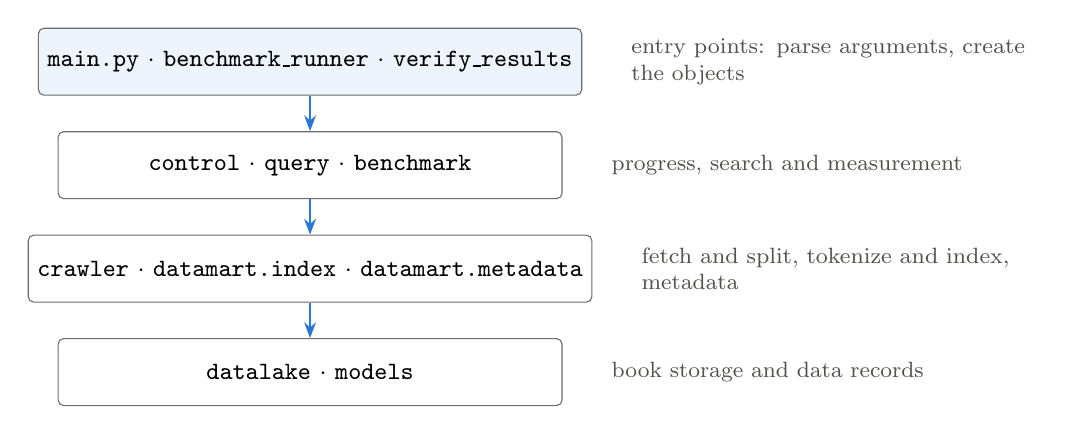
\begin{tikzpicture}[font=\small,
  layer/.style={draw=ink!60,rounded corners=2pt,minimum width=6.4cm,minimum height=0.85cm,fill=white},
  arr/.style={-{Stealth[length=2mm]},thick,draw=accent}]
  \node[layer,fill=notebg] (a) {\code{main.py} $\cdot$ \code{benchmark\_runner} $\cdot$ \code{verify\_results}};
  \node[layer,below=0.45cm of a] (b) {\code{control} $\cdot$ \code{query} $\cdot$ \code{benchmark}};
  \node[layer,below=0.45cm of b] (c) {\code{crawler} $\cdot$ \code{datamart.index} $\cdot$ \code{datamart.metadata}};
  \node[layer,below=0.45cm of c] (d) {\code{datalake} $\cdot$ \code{models}};
  \foreach \x/\y in {a/b,b/c,c/d} \draw[arr] (\x) -- (\y);
  \node[right=0.5cm of a,text width=5.2cm,color=muted,font=\footnotesize] {entry points: parse arguments, create the objects};
  \node[right=0.5cm of b,text width=5.2cm,color=muted,font=\footnotesize] {progress, search and measurement};
  \node[right=0.5cm of c,text width=5.2cm,color=muted,font=\footnotesize] {fetch and split, tokenize and index, metadata};
  \node[right=0.5cm of d,text width=5.2cm,color=muted,font=\footnotesize] {book storage and data records};
\end{tikzpicture}
\caption{Layers. Each one only uses the layers below it.}
\end{figure}

\subsection{Design principles applied throughout}
\begin{table}[H]
\centering\small
\begin{tabularx}{\linewidth}{@{}p{3.1cm} Y Y@{}}
\toprule
Principle & Where & Why \\
\midrule
Abstract base classes & \code{Datalake} and \code{InvertedIndex} (\code{abc.ABC}) & Every structure offers the same methods, so the pipeline, the search and the benchmarks treat them alike. \\
Dependencies passed in & Paths, the clock of \code{TimeBasedDatalake}, the Mongo database name & Tests and benchmarks use temporary folders, a simulated clock and \code{search\_engine\_bench} without touching the code. \\
One way to write a file & \code{Datalake.\_write\_file}: subclasses decide \emph{where}, the base decides \emph{how}. & The delicate part (the atomic write) exists only once for the three layouts. \\
Atomic writes & Datalake files, \code{inverted\_index.json}, term files, CSV results & A crash never leaves a half-written file under its final name. \\
Idempotence & \code{INSERT OR REPLACE}, sets in \code{add\_document}, \code{\$addToSet}, marks that check first & Processing a book twice after a failure adds nothing. \\
Mark after doing & \code{mark\_as\_downloaded} and \code{mark\_as\_indexed} come last & The control layer never claims something that was not written. \\
Immutable records & \code{RawBook}, \code{BookLocation}, \code{BookMetadata}: frozen dataclasses with \code{\_\_slots\_\_} & Plain data that cannot be changed by accident, and small in memory. \\
\bottomrule
\end{tabularx}
\caption{Design principles and where they appear in the code.}
\end{table}

\subsection{Project organisation}

\subsubsection{Folder tree}
\begin{lstlisting}[style=shell]
stage_1/
|-- README.md                  overview of the group project
|-- docker-compose.yml         MongoDB 8.2 server shared by the three implementations
|-- shared/                    COMMON CONTRACT (Java, Python and C++)
|   |-- SPEC.md, book_ids.txt, queries.txt, stopwords.txt
|-- sample_dataset/            first 15 books, raw (input) and split (expected output)
`-- python/
    |-- requirements.txt       requests, pymongo
    `-- stage_1/               <- the Python implementation (run everything from here)
        |-- README.md          user guide of the module
        |-- docs/              this report; report/ holds its LaTeX source and scripts
        |-- src/main/bigdata/
        |   |-- main.py        command line: pipeline | search | status
        |   |-- models.py      RawBook, BookLocation, BookMetadata (dataclasses)
        |   |-- crawler/       client.py (HTTP), splitter.py (markers, offline read)
        |   |-- datalake/      base.py, book_based.py, range_based.py, time_based.py
        |   |-- datamart/metadata/  parser.py, repository.py (SQLite)
        |   |-- datamart/index/     tokenizer.py, base.py, monolithic.py, hierarchical.py,
        |   |                       mongo.py, in_memory.py
        |   |-- query/         search_service.py (AND)
        |   |-- control/       state_manager.py (ControlLayer)
        |   `-- benchmark/     benchmark_runner.py, datalake_/index_/metadata_benchmark.py,
        |                      runner.py, books.py, csv_results.py, verify_results.py
        |-- src/test/          39 tests (pytest), one package per source package
        |-- data/              (generated, ignored by git) datalake, datamarts, control
        `-- benchmarks/        results/{real,synthetic}/*.csv (committed), data/ (ignored)
\end{lstlisting}

\subsubsection{Size of the code}
\begin{table}[H]
\centering\small
\begin{tabularx}{\linewidth}{@{}l Y@{}}
\toprule
Item & Amount \\
\midrule
Production modules & 26 (about 2,900 lines with comments and docstrings) \\
Test modules & 14 (about 630 lines), 39 tests \\
External dependencies & \code{requests} 2.32, \code{pymongo} 4.18; \code{pytest} for the tests; \code{matplotlib} only for this report's charts \\
\bottomrule
\end{tabularx}
\end{table}

\subsubsection{Where each part of the state lives}
\begin{table}[H]
\centering\small
\begin{tabularx}{\linewidth}{@{}p{2.3cm} Y p{5.4cm}@{}}
\toprule
State & File or database & Written by \\
\midrule
Book text & \code{data/datalake/\{book,range,time\}/\ldots} & \code{Datalake.save} \\
Metadata & \code{data/datamarts/metadata.db} (table \code{books}) & \code{MetadataRepository.save\_all} \\
Monolithic index & \code{data/datamarts/} \code{inverted\_index.json} & \code{MonolithicJsonIndex.flush} \\
Hierarchical index & \code{data/datamarts/inverted\_index/} \code{<L>/<term>.txt} & \code{HierarchicalFolderIndex.flush} \\
Mongo index & database \code{search\_engine}, collection \code{inverted\_index} & \code{MongoInvertedIndex.flush} \\
Progress & \code{data/control/downloaded\_books.txt}, \code{indexed\_books.txt} & \code{ControlLayer.mark\_as\_*} \\
Benchmark results & \code{benchmarks/results/\{real,synthetic\}/} \code{python\_<experiment>.csv} & \code{csv\_results.write\_csv} \\
\bottomrule
\end{tabularx}
\end{table}

% ================================================================ 3
\section{Design decisions}\label{sec:decisions}

\subsection{Structures selected for the final implementation}
The Python pipeline keeps every structure up to date, so choosing one does not change what is
stored; it decides which structure a search engine built on this layer should rely on.

\textbf{Datalake.} \pending{the layout chosen and why, from the datalake results of
Section~\ref{sec:bench}: write throughput, lookup cost, incremental detection, recovery and storage
overhead.}

\textbf{Inverted index.} \pending{the index chosen and why, from the index results of
Section~\ref{sec:bench}: build, query, update, memory and disk.}

\subsection{Implementation decisions}
\begin{description}[style=nextline,leftmargin=0pt,itemsep=6pt]
  \item[The pipeline writes the three structures at once.] Every book goes to the three datalakes
        and the three indexes in the same pass. One \code{pipeline 200} run fills everything the
        benchmarks and the comparison need, and the structures can never drift apart, because they
        are built from the same book in the same step. The price is that each book is written six
        times; for 200 books this is a matter of minutes, and the download dominates anyway.
  \item[Standard library, plus \code{requests} and \code{pymongo}.] SQLite comes with Python
        (\code{sqlite3}), as do JSON, paths, \code{tracemalloc} and timing. Keeping the dependencies to
        two well-known packages makes the module easy to install on any machine, which matters
        because the official benchmarks were run on a different computer than the one used to
        write the code.
  \item[A tokenizer that walks the text character by character.] \code{tokenize} is a loop that
        compares each character with the ranges \code{A}--\code{Z}, \code{a}--\code{z} and
        \code{0}--\code{9}, exactly as SPEC section 5 describes. A regex such as \code{\textbackslash w+}
        or \code{str.lower()} would follow Unicode rules (accented letters, the underscore) and give
        different terms from Java and C++. With the loop, the index of the 200 books has exactly the
        129,356 terms and 1,581,064 postings of the reference.
  \item[Atomic writes with \code{.tmp} and \code{os.replace}.] Datalake files, the monolithic JSON
        and each hierarchical term file are first written to \code{<name>.tmp} and then moved over
        the final name. \code{os.replace} is atomic within one file system on Linux and Windows, so a
        file under its final name is always complete, and a \code{.tmp} never counts as a saved book.
        The datalake recovery benchmark relies on it: it simulates a crash by leaving bodies as
        \code{.tmp}.
  \item[Save each book before marking it (SPEC section 8).] The three indexes are flushed after
        every book, and only then is the id appended to \code{indexed\_books.txt}. Flushing the
        monolithic JSON after every book costs time, since the whole file is rewritten, but it is
        what makes the control layer truthful: if the run stops, every book marked as indexed is
        really on disk, and the worst case is indexing one book again, which adds nothing.
  \item[A control layer that trims a half-written line.] Ids are appended one per line. If the
        process dies in the middle of an append, the file can end in a fragment such as \code{13}.
        \code{ControlLayer} only counts lines that end in \code{\textbackslash n} and truncates such a
        fragment when it starts, as Java's \code{ControlFiles} does, so the next append cannot glue
        it to another id (\code{13} + \code{84} = \code{1384}).
  \item[\code{JavaRandom} and \code{java\_shuffle}.] Python's \code{random} does not produce Java's
        sequence for the same seed. Where the comparison between languages depends on random
        choices, the lookup order of \code{datalake\_lookup} and the rows picked by
        \code{metadata\_query} (both with seed 42), Python uses a port of \code{java.util.Random}
        (the same 48-bit linear congruential generator and \code{nextInt} rejection loop) and of
        \code{Collections.shuffle}. They were checked against the JDK and give exactly its output.
  \item[\code{\$addToSet} in MongoDB.] A flush sends one upsert per pending term, all in one
        unordered \code{bulk\_write}, with \code{\$addToSet} and \code{\$each}. Adding the same book
        twice leaves the posting list unchanged, which keeps the index correct when a book is
        processed again after an interruption. Because Mongo does not keep arrays sorted,
        \code{postings} sorts what it reads.
  \item[Check every index against an in-memory one.] After measuring, each index benchmark calls
        \code{verify()}, a port of Java's \code{IndexBenchmark.verify}: the index must give the same
        posting lists as an in-memory index built from the same books, for the query terms and the
        first 20 terms of the first and last book, and the same answer to every query. A benchmark
        that measured a wrong index stops with an error instead of writing numbers.
\end{description}

% ================================================================ 4
\section{Implementation: modules and classes}
For each module: what it is, what it is responsible for, its important functions, and the reason
for its design. The order follows the path of the data. All paths are relative to
\code{src/main/bigdata/}.

% ---------------------------------------------------------------- models
\subsection{Module \code{models}: the data that travels}
\cls{RawBook}{frozen dataclass}
A downloaded book: \code{id}, \code{header} and \code{body}. It is what the splitter returns and what
the datalakes save.

\cls{BookLocation}{frozen dataclass}
Where a book is stored: its id and the paths of its header and body files.

\cls{BookMetadata}{frozen dataclass}
A row of the \code{books} table: id, title, author, language, release date and the two paths.
\why{\code{frozen=True} makes the records impossible to change by accident once created, and
\code{slots=True} keeps them small when the benchmarks hold hundreds of thousands of them.}

% ---------------------------------------------------------------- crawler
\subsection{Package \code{crawler}: fetching and splitting}
\cls{client.download\_raw\_text}{function}
Downloads \code{https://www.gutenberg.org/cache/epub/<ID>/pg<ID>.txt} with \code{requests} (30~s
timeout), decodes it as UTF-8 and turns \code{\textbackslash r\textbackslash n} into
\code{\textbackslash n}. A non-200 answer raises \code{DownloadError}.

\cls{splitter.split\_header\_body}{function}
Finds the first line that contains the START marker and the first END marker after it, with
case-sensitive regexes that accept \code{THE} and \code{THIS}. The header is everything before the
START line and the body everything between the two marker lines, both trimmed. A missing marker
raises \code{MarkerNotFoundError}.

\cls{splitter.fetch\_book, fetch\_book\_offline}{functions}
Download (or read \code{<dir>/pg<ID>.txt}) and split, returning \code{None} instead of raising, so
the pipeline only has to check one value. The offline variant reads the same raw bytes Gutenberg
serves, so everything after it is identical to an online run.
\why{The split is a pure function of the text: it can be tested without network, and the online
and offline paths share it.}

% ---------------------------------------------------------------- datalake
\subsection{Package \code{datalake}: storing the books}
\cls{Datalake}{abstract base class, \code{base.py}}
The common interface: \code{name}, \code{save(book)}, \code{locate(id)} and
\code{list\_book\_ids()}. It also holds the only file writer, \code{\_write\_file}: create the folder,
write \code{<name>.tmp}, \code{os.replace} it over \code{<name>}, and delete the \code{.tmp} if
anything fails. A book counts as saved only when its header and body both exist as regular files.

\cls{BookBasedDatalake}{layout \code{book}}
\code{<ID>/header.txt} and \code{<ID>/body.txt}. \code{locate} computes the path from the id; listing
keeps only canonical numeric folder names.

\cls{RangeBasedDatalake}{layout \code{range}}
\code{<START>-<END>/<ID>.\{header,body\}.txt}, with \code{START = (id // 1000) * 1000} and five
digits. Listing ignores files whose id does not belong to the range of their folder.

\cls{TimeBasedDatalake}{layout \code{time}}
\code{YYYYMMDD/HH/<ID>.\{header,body\}.txt}, with the time given by a clock passed to the
constructor (\code{datetime.now} by default). The path cannot be computed from the id, so
\code{locate} searches the hour folders from the newest, and \code{list\_book\_ids} removes repeated
ids.
\why{Passing the clock in lets the benchmark use a simulated one (10 books per hour from 1~January
2026, UTC, as Java's \code{SimulatedClock}), so every repetition creates exactly the same folders.}

% ---------------------------------------------------------------- metadata
\subsection{Package \code{datamart.metadata}: metadata in SQLite}
\cls{parser.parse\_metadata}{function}
Applies the four multi-line regexes of SPEC section 4 to the header and returns a dictionary with
\code{title}, \code{author}, \code{release\_date} and \code{language}. Each value is the first match,
first line only, trimmed; a missing or empty value is \code{None}, which SQLite stores as NULL. The
release date drops whatever follows a bracket, such as \code{[eBook \#1342]}.

\cls{repository.MetadataRepository}{class}
Opens (or creates) \code{metadata.db} with the SPEC schema, optionally without the \code{author}
and \code{title} indexes (the \code{sqlite\_no\_index} variant of the benchmark).
\code{save\_all(rows)} inserts a batch with \code{executemany} and \code{INSERT OR REPLACE}, in one
transaction; \code{find\_by\_id}, \code{find\_by\_author} and \code{find\_by\_title} return
\code{BookMetadata} records, the last two ordered by \code{book\_id}.
\why{\code{INSERT OR REPLACE} makes saving a book twice harmless, and one commit per batch is what
makes bulk inserts fast in SQLite.}

% ---------------------------------------------------------------- index
\subsection{Package \code{datamart.index}: the inverted index}
\cls{tokenizer.tokenize}{function}
The loop of SPEC section 5 (Section~\ref{sec:decisions}). It returns a \code{set}, since each book
contributes each term once. The stopwords are read once, when the module is imported, from
\code{shared/stopwords.txt}.

\cls{InvertedIndex}{abstract base class, \code{base.py}}
\code{add\_document(id, terms)}, \code{postings(term)} (sorted ids), \code{flush()},
\code{clear()}, \code{disk\_usage\_bytes()} and \code{close()}. \code{add\_document} only touches
memory; nothing is persistent until \code{flush}.

\cls{InMemoryInvertedIndex}{class, structure \code{memory}}
A dictionary of sets. It is never persisted: it is the reference against which \code{verify()}
checks the other three.

\cls{MonolithicJsonIndex}{class, structure \code{monolithic}}
Loads \code{inverted\_index.json} when created and keeps the whole index in memory. \code{flush}
serialises it with sorted keys, sorted ids and no spaces (\code{separators=(',', ':')}), writes it to
\code{inverted\_index.json.tmp} and moves it into place. The bytes are identical to Java's file.

\cls{HierarchicalFolderIndex}{class, structure \code{hierarchical}}
One file per term in \code{<root>/<FIRST LETTER>/<term>.txt}, one id per line; terms that start with
a digit go to the folder of that digit. \code{add\_document} accumulates pending ids;
\code{flush} reads each changed term's file, merges, and rewrites it (\code{.tmp} + move) only if
some id was new. \code{postings} reads a single file and adds what is pending.

\cls{MongoInvertedIndex}{class, structure \code{mongo}}
Collection \code{inverted\_index} with a unique index on \code{term}, created in the constructor,
which also checks that the server answers within 3~s. \code{flush} sends all pending terms in one
unordered \code{bulk\_write} of upserts with \code{\$addToSet}. \code{disk\_usage\_bytes} asks for an
\code{fsync} and returns \code{storageSize + totalIndexSize} from \code{collStats}.
\why{The three persistent indexes keep pending work in memory and only write in \code{flush}, so the
caller decides when the disk is touched: once per book in the pipeline, once per build in the
benchmark.}

% ---------------------------------------------------------------- query
\subsection{Package \code{query}: the search}
\cls{search\_service.search}{function}
Tokenizes the query, returns an empty list if no term is left, asks the index for every posting
list (stopping at the first empty one), sorts them by length and intersects them with two
pointers, the shortest first, so every step works on the smallest possible list. The result is
sorted, as SPEC section 7 requires, and works with any \code{InvertedIndex}.

% ---------------------------------------------------------------- control
\subsection{Package \code{control}: progress and recovery}
\cls{state\_manager.ControlLayer}{class}
Owns \code{downloaded\_books.txt} and \code{indexed\_books.txt}. \code{is\_downloaded} and
\code{is\_indexed} read the complete lines of the file; \code{mark\_as\_downloaded} and
\code{mark\_as\_indexed} append an id only if it is not there yet. When created, it truncates a last
line left without \code{\textbackslash n}. Valid ids follow the datalake's rule (\code{0} or no
leading zeros, at most 9 digits), and a Windows \code{\textbackslash r} is ignored.
\why{The files are the only memory of the progress between runs, so they are read from disk every
time instead of being cached, and they are append-only.}

% ---------------------------------------------------------------- cli
\subsection{The command line: \code{main.py}}
\code{python -m src.main.bigdata.main} with three sub-commands (\code{argparse}):
\code{pipeline [steps] [-{}-offline-source DIR]}, \code{search WORDS...} and \code{status}. The
pipeline loop is described in Section~\ref{sec:life}. A book that cannot be fetched or split counts as an
error and is retried in the next run; one already indexed counts as skipped. MongoDB is optional:
if the connection fails, the run continues with the other two indexes and says so. \code{search}
reads the monolithic index.

Known limitation: a book that was downloaded but not indexed when a run stopped is downloaded again
on the next run, instead of being read from the datalake as Java does. The result is the same, but
in the \code{time} layout the book can then exist in two hour folders; \code{locate} returns the
newest and \code{list\_book\_ids} reports the id once.

% ---------------------------------------------------------------- benchmark
\subsection{Package \code{benchmark}}
\cls{runner}{module}
\code{measure(experiment, structure, N, setup, task)} runs \code{setup} (not timed) and
\code{task} (timed with \code{time.perf\_counter\_ns}) 2 + 5 times and returns one \code{BenchmarkRow}
per measured run. \code{BenchmarkRow} formats the CSV line with at most 3 decimals.
\code{JavaRandom} and \code{java\_shuffle} also live here.

\cls{csv\_results}{module}
Writes a whole CSV with LF line endings to \code{<file>.tmp} and moves it into place.

\cls{books}{module}
\code{from\_datalake} reads every book of a \code{book} datalake in ascending id order (SPEC 10.1);
\code{synthetic} and \code{synthetic\_zipf} generate books from a seed.

\cls{datalake\_benchmark, index\_benchmark, metadata\_benchmark}{modules}
The 12 experiments (Section~\ref{sec:bench}) and their checks.

\cls{benchmark\_runner}{entry point}
With a datalake path, the real mode (10 CSVs in \code{results/real/}); without it, the synthetic
mode (12 CSVs in \code{results/synthetic/}).

\cls{verify\_results}{entry point}
Checks the CSVs against the exact values of SPEC section 10 (Section~\ref{sec:checks}).

% ================================================================ 5
\section{Testing strategy}
\code{pytest src/test} runs 39 tests in 14 modules, which mirror the packages of the code. They need
no network and no database server, and write only to temporary folders.

\begin{table}[H]
\centering\small
\begin{tabularx}{\linewidth}{@{}l Y r@{}}
\toprule
Module & What it checks & Tests \\
\midrule
\code{crawler/test\_splitter} & The header is what precedes START, the body what lies between the markers, neither contains a marker, and the result is a (header, body) pair. & 5 \\
\code{control/test\_state\_manager} & Marks written once; a half-written last line ignored and truncated, so the next id is not glued to it; a file without any newline; \code{\textbackslash r\textbackslash n}, garbage and leading zeros. & 5 \\
\code{datalake/test\_range\_based} & The range folder of ids 0, 999, 1530 and 2000. & 4 \\
\code{datamart/test\_tokenizer} & Lowercasing, accented characters as separators, stopwords and the minimum length. & 4 \\
\code{datamart/test\_metadata} & Title, author and language extracted; a missing release date is \code{None}; the four keys always present. & 3 \\
\code{datamart/test\_hierarchical\_index} & A flush sorts out-of-order ids and removes duplicates. & 2 \\
\code{datalake/test\_book\_and\_time\_based} & The \code{book} paths and content, \code{locate} and listing, a body left as \code{.tmp} not counted; the \code{time} layout with the simulated clock (10 books per hour) and a repeated book located in its newest folder and listed once. & 5 \\
\code{benchmark/test\_java\_random} & \code{JavaRandom.next\_int} and \code{java\_shuffle} against values produced by the JDK with seed 42. & 3 \\
\code{benchmark/test\_index\_verify} & \code{verify()} accepts a correct index and stops on an index that loses a posting or a book. & 3 \\
Other five modules & Import checks of the runner, the metadata repository, the Mongo, monolithic and search modules. & 5 \\
\bottomrule
\end{tabularx}
\caption{The \code{pytest} suite.}
\end{table}

\textbf{MongoDB.} The unit suite has no test that needs a server: \code{test\_mongo\_index} only
checks that the module imports. The Mongo index is exercised against a real server by the
benchmarks, where every experiment checks it with \code{verify()}, and by the pipeline checks of
Section~\ref{sec:checks}.

\subsection{Checks beyond the unit tests}\label{sec:checks}
Most of the evidence that the Python module is correct comes from checks that run on the real data.
\begin{itemize}
  \item \textbf{\code{verify()} in the five index experiments.} After \code{index\_build} and
        \code{index\_update}, on the reopened index in \code{index\_query} and \code{index\_memory},
        and before writing the rows of \code{index\_disk}, each backend is compared with an
        in-memory index built from the same books. A fresh index is also checked to be empty
        (no files, no postings for the query terms) every time an experiment starts from an empty index.
  \item \textbf{Datalake checks.} \code{datalake\_lookup} requires every id to be found;
        \code{datalake\_incremental} requires the detected ids to be exactly the new ones;
        \code{datalake\_recovery} requires recovered = damaged, lost = 0 and duplicates = 0, computed
        on the final state of the folder. The metadata experiments check the number of inserted
        rows and that the 1,000 queries of each type return at least 1,000 rows.
  \item \textbf{\code{verify\_results}.} Checks the committed CSVs: the exact storage, recovery,
        incremental and index counts, and that every experiment has its 5 runs. It exits with code
        1 if anything fails.
  \item \textbf{Parity with Java, checked on the output of \code{pipeline 200}.} The monolithic
        index has 8,893,537 bytes, 129,356 terms and 1,581,064 postings; the hierarchical index has
        129,356 files and 7,251,967 bytes; every posting list is sorted, without duplicates and
        without \code{\textbackslash r}, and each term file equals its JSON entry. These numbers are
        identical to Java's. The Mongo collection of \code{search\_engine} has 129,356 documents and
        1,581,064 postings. No file of the datalake contains a \code{\textbackslash r}, and the three
        layouts hold 200 headers and 200 bodies each.
  \item \textbf{Java's random sequence.} \code{JavaRandom} and \code{java\_shuffle} were run next to
        the JDK on a 200-id shuffle and 3,000 \code{nextInt} calls: the output is exactly the same.
  \item \textbf{End to end.} The real mode of the runner on the 15 books of
        \code{sample\_dataset/book} finishes without errors, with the three index backends, and
        recovers 2 / 0 / 0 books.
\end{itemize}

% ================================================================ 6
\section{Setup and execution}

\subsection{Requirements}
\begin{itemize}
  \item Python 3.10 or newer, and \code{pip}.
  \item \code{requests} and \code{pymongo} (\code{python/requirements.txt}); \code{pytest} for the tests.
  \item MongoDB, only for the \code{mongo} index: \code{docker compose up -d} at the repository root
        starts the group's MongoDB~8.2 on \code{127.0.0.1:27017}. Without it, the pipeline and the
        benchmarks skip that index with a warning.
\end{itemize}

\subsection{Setup and tests}
From \code{python/stage\_1/}:
\begin{lstlisting}[style=shell]
python -m venv venv
source venv/bin/activate              # Windows: venv\Scripts\activate
pip install -r ../requirements.txt pytest
pytest src/test                       # 39 passed
\end{lstlisting}

\subsection{Quick test without network: the sample dataset}\label{sec:quick}
\code{sample\_dataset/raw/} holds the first 15 books of the dataset exactly as Gutenberg serves
them. Starting from an empty \code{data/}:
\begin{lstlisting}[style=shell]
python -m src.main.bigdata.main pipeline 15 --offline-source ../../sample_dataset/raw
python -m src.main.bigdata.main search whale island
[INFO] Found 3 books: [76, 84, 2701]
\end{lstlisting}
A later online \code{pipeline} finds those 15 books already indexed and downloads only the other 185.

\subsection{Commands}
\begin{table}[H]
\centering\small
\begin{tabularx}{\linewidth}{@{}p{5.2cm} Y@{}}
\toprule
Command (\code{python -m src.main.bigdata.main \ldots}) & What it does \\
\midrule
\code{pipeline [steps]} & Processes up to \code{steps} books not yet indexed, in the order of \code{book\_ids.txt} (all by default). \\
\code{pipeline [steps] -{}-offline-source DIR} & The same, reading \code{DIR/pg<ID>.txt}. \\
\code{search WORDS...} & AND search on the monolithic index; prints the ids. \\
\code{status} & Books in the dataset, downloaded, indexed, and pending (not indexed). \\
\bottomrule
\end{tabularx}
\end{table}
A step is one book (download and indexing), so \code{pipeline 200} here does what
\code{pipeline 400} does in Java and C++. With the whole dataset, \code{status} reports 200
downloaded, 200 indexed and 0 pending.

\subsection{Running the benchmarks}
The real mode reads a \code{book} datalake: \code{data/datalake/book} after \code{pipeline 200}, or
Java's, which is byte-for-byte the same. Run the two modes one after the other, then check the CSVs:
\begin{lstlisting}[style=shell]
python -m src.main.bigdata.benchmark.benchmark_runner data/datalake/book > benchmarks/bench_real.log 2>&1
python -m src.main.bigdata.benchmark.benchmark_runner > benchmarks/bench_synthetic.log 2>&1
python -m src.main.bigdata.benchmark.verify_results
\end{lstlisting}
Both logs must list the backends \code{['monolithic', 'hierarchical', 'mongo']}. The CSVs of each
block (datalake, metadata, index) are written when the block ends, so the machine must not sleep
during the run, which takes hours.

\textbf{Windows and Linux.} The commands are the same on both (on Windows, \code{venv\textbackslash
Scripts\textbackslash activate}). The difference is speed: each repetition of the hierarchical index
experiments creates and deletes about 129,000 small files, which is far slower on NTFS with an
antivirus scanning every new file, and a folder synchronised by OneDrive makes it worse. The
official results were therefore produced on Linux.

% ================================================================ 7
\section{Benchmarks and results}\label{sec:bench}

\subsection{Methodology}
\begin{itemize}
  \item \textbf{Warm-ups and measured runs:} 2 discarded repetitions and 5 measured ones, timed with
        \code{time.perf\_counter\_ns}. Tables give the \textbf{median} of the 5.
  \item \textbf{Setup outside the measurement:} deleting folders, filling the datalake or the
        index that an experiment starts from, opening connections and tokenizing the books happen
        in the untimed setup. What is timed: saving the books (\code{datalake\_write}); every
        \code{locate} (\code{datalake\_lookup}); listing the ids minus the known ones
        (\code{datalake\_incremental}); listing and saving the missing books
        (\code{datalake\_recovery}); the batches of 1,000 rows (\code{metadata\_insert}); 1,000
        queries of one type (\code{metadata\_query}); \code{add\_document} of the N books plus one
        flush (\code{index\_build}); 100 rounds of the 10 queries of \code{queries.txt}
        (\code{index\_query}); adding the last 10\% of the books with one flush per book
        (\code{index\_update}).
  \item \textbf{Same data and order as Java:} the books in ascending id order, N as a prefix,
        the 10\% splits of Java, and \code{JavaRandom(42)} for the lookup order and the metadata
        queries. The \code{time} layout uses a simulated clock of 10 books per hour.
  \item \textbf{Verification:} every experiment checks its result (Section~\ref{sec:checks}); a
        failed check stops the run before any CSV is written.
  \item \textbf{\code{index\_memory}:} measured with \code{tracemalloc}. It is the net difference of
        the live memory allocated through Python's allocator, after \code{gc.collect()}, between
        before and after building the index (\code{heap\_after\_build}) and between before and
        after reopening it (\code{heap\_after\_open}). It does not include the memory of
        \code{mongod}, nor what C libraries allocate outside Python's allocator, nor the books, which
        were loaded before tracing started. Negative values are kept, as in Java. It is not
        comparable in absolute value with the JVM heap that Java reports, only in how it grows
        with N.
\end{itemize}

\begin{note}
\textbf{Environment.} Same Linux machine as the Java run (12 threads, 15~GB RAM, NVMe SSD), Python
\pending{version}, MongoDB~8.2 in Docker (local). Absolute values depend on the machine; what
matters are the ratios and how they change as N grows.
\end{note}

\subsection{Data: real and synthetic}
\begin{itemize}
  \item \textbf{Real books (SPEC 10.1)} for the datalake and index experiments: the 200 books of
        \code{shared/book\_ids.txt}, read from a \code{book} datalake (129.0~MB). The datalake uses
        all 200; the index uses the prefixes of 50, 100 and 200 books, with exactly 58,834,
        78,820 and 129,356 terms.
  \item \textbf{Generated metadata (SPEC 10.2)} for the metadata experiments: 1,000, 10,000 and
        100,000 rows built without random numbers (every author has 10 books and every title 2),
        identical in the three languages.
  \item \textbf{Synthetic books (SPEC 10.3):} the synthetic mode also runs the datalake and index
        experiments on 200 generated books (5,000 Zipf-distributed words from a vocabulary of
        5,000). They come from Python's \code{random}, so they are a Python-only reference and are
        not compared with the other languages.
\end{itemize}

\subsection{Datalake benchmark}
Data: the 200 real books, the same bytes in the three layouts.

\begin{table}[H]
\centering\small
\begin{tabularx}{\linewidth}{@{}l Y l@{}}
\toprule
Experiment & What exactly is measured & Metrics \\
\midrule
\code{datalake\_write} & Saving the 200 books into an empty datalake. & elapsed (ms), throughput (books/s) \\
\code{datalake\_lookup} & \code{locate()} of every id, in Java's shuffled order (seed 42). & elapsed, per\_lookup (\us) \\
\code{datalake\_incremental} & With 180 known and 20 new books: \code{list\_book\_ids()} minus the known ids. & elapsed, detected \\
\code{datalake\_recovery} & 1 book in 10 has its body left as \code{.tmp}; listing and saving the missing ones again. & elapsed, recovered, lost, duplicates \\
\code{datalake\_storage} & After saving everything: files, folders, fullest folder, bytes and allocated bytes (4~KB blocks). & files, directories, \ldots \\
\bottomrule
\end{tabularx}
\end{table}

\begin{figure}[H]
\centering
\pythonfigure{datalake}{\linewidth}
\caption{Datalake with the 200 real books (median of 5 runs).}
\end{figure}

\begin{table}[H]
\centering\small
\pythontable{datalake}
\caption{Datalake with the 200 real books (median of 5 runs).}
\end{table}

\pending{comment on the datalake results.}

\subsection{Metadata benchmark}
Data: the generated rows of SPEC 10.2. \code{metadata\_insert} times inserting N rows in batches of
1,000, one transaction each, into an empty database; \code{metadata\_query} times 1,000 queries by
id, by author and by title, picked with \code{JavaRandom(42)} among existing values. Each runs on
\code{sqlite} (the SPEC schema) and \code{sqlite\_no\_index} (without the author and title
indexes).

\begin{figure}[H]
\centering
\pythonfigure{metadata}{\linewidth}
\caption{Metadata in SQLite with 1,000, 10,000 and 100,000 rows (median of 5 runs).}
\end{figure}

\begin{table}[H]
\centering\small
\pythontable{metadata}
\caption{Metadata: insert throughput and average time per query (median of 5 runs).}
\end{table}

\pending{comment on the metadata results.}

\subsection{Inverted-index benchmark}
Data: the prefixes of 50, 100 and 200 real books, tokenized once before any measurement, so the
tokenizer is not in any timing.

\begin{figure}[H]
\centering
\pythonfigure{index_build_query}{\linewidth}
\caption{Building the index and answering the AND queries (median of 5 runs).}
\end{figure}

\begin{figure}[H]
\centering
\pythonfigure{index_update}{0.62\linewidth}
\caption{Cost of adding one book, with a flush per book, to an index that already holds 90\% of N.}
\end{figure}

\begin{figure}[H]
\centering
\pythonfigure{index_disk_memory}{\linewidth}
\caption{Disk usage and Python heap (\code{tracemalloc}) with N = 200.}
\end{figure}

\begin{table}[H]
\centering\small
\resizebox{\linewidth}{!}{\pythontable{index}}
\caption{Inverted index (median of 5 runs). Query: average per AND query; update: per added book;
heap: \code{tracemalloc}, after building and after reopening.}
\end{table}

\pending{comment on the index results.}

\subsection{Comparison with Java and C++}\label{sec:lang}
The three implementations follow the same SPEC, measure the same books and write the same CSV
format, so their results can be put side by side. Java and Python were measured on the same Linux
machine; C++ was measured on macOS on Apple Silicon. A difference between Java and Python is
therefore a difference of language and implementation, while a difference with C++ also includes
the machine and the operating system.

A first attempt to produce the Python results on Windows~11 was many times slower than the Linux
run: most of the time went into creating and deleting the $\sim$129,000 small files of the
hierarchical index on NTFS, with Microsoft Defender scanning each one. For that reason the official
Python results were taken on Linux, on the same machine as Java's.

\begin{figure}[H]
\centering
\pythonfigure{lang_datalake}{\linewidth}
\caption{Datalake in the three languages, 200 real books (median of 5 runs).}
\end{figure}

\begin{figure}[H]
\centering
\pythonfigure{lang_index}{\linewidth}
\caption{Inverted index in the three languages, N = 200 (median of 5 runs, log scale).}
\end{figure}

\begin{figure}[H]
\centering
\pythonfigure{lang_metadata}{\linewidth}
\caption{Metadata in the three languages, 100,000 generated rows (median of 5 runs).}
\end{figure}

\begin{table}[H]
\centering\small
\pythontable{lang_summary}
\caption{Key results in the three languages (median of 5 runs). The byte and term counts must be
identical; the times are not expected to be.}
\end{table}

\pending{comment on the comparison: what is a difference of language and what is a difference of
machine.}

\subsection{Summary: which structure to choose}
\pending{summary table and choice of structures, once all the results are in.}

% ================================================================ 8
\section{Conclusions and future improvements}

\subsection{Conclusions}
The Python implementation delivers the complete Stage~1 data layer: crawler, datalake, metadata and
inverted-index datamarts, AND search and a control layer that survives interruptions. One pipeline
run fills the three datalake layouts and the three indexes, and its output matches the Java
implementation byte for byte. The 12 benchmark experiments run with the methodology of the SPEC,
check their own results, and are checked again by \code{verify\_results}. \pending{the main
conclusions from the results.}

\subsection{Limitations and future improvements}
\begin{itemize}
  \item \textbf{The cost of the interpreter in loops.} The tokenizer walks every character of every
        book in Python code, and the hierarchical index reads and writes files term by term. Both
        are interpreted loops, much slower than the same loops compiled in Java or C++. Moving the
        tokenizer to a compiled routine (or vectorising it over bytes) would keep the SPEC rules and
        remove most of that cost.
  \item \textbf{Tokenizing in parallel.} Books are independent, so tokenization could use
        \code{multiprocessing} (one process per core, avoiding the global interpreter lock) before
        the single-threaded indexing step.
  \item \textbf{Grouping writes.} The pipeline flushes the three indexes after every book, which is
        what makes the control layer safe, but rewrites the whole monolithic JSON 200 times.
        Flushing every K books and marking those K books together would keep the guarantee of SPEC
        section 8 with far fewer writes; for the hierarchical index, writing the term files of
        several books at once would reduce the number of file operations.
  \item \textbf{Memory limits of the monolithic index.} The whole index lives in a dictionary of
        Python sets, whose objects are much larger than the integers they hold. With thousands of
        books the index would no longer fit comfortably in memory, and the hierarchical or Mongo
        index (which keep only the pending book in memory) would become necessary.
  \item \textbf{Re-download on resume.} A book downloaded but not indexed when a run stops is
        downloaded again instead of being read from the datalake. Reading it back would match
        Java's ``index what is downloaded first'' and avoid a second copy in the \code{time} layout.
  \item \textbf{More unit tests.} The metadata repository, the monolithic and Mongo indexes and the
        search are covered by the benchmark checks and the pipeline output, but their unit tests
        only check the import; behavioural tests for them (Mongo ones skipped without a server)
        would catch regressions earlier.
\end{itemize}

\end{document}
